\documentclass[12pt]{article}
\usepackage[margin=1in]{geometry}
\usepackage{graphicx}
\usepackage{booktabs}
\usepackage{amsmath}
\usepackage{natbib}
\usepackage{setspace}
\onehalfspacing

\title{Replication of Table 1 from Arkhangelsky et al.\ (2021)}
\author{Lauren Taylor}
\date{\today}

\begin{document}
\maketitle

\section{The Original Paper}

This study replicates \textbf{``Synthetic Difference-in-Differences''} written by
\textbf{Dmitry Arkhangelsky, Susan Athey, David A.\ Hirshberg, Guido W.\ Imbens,
and Stefan Wager} and published in the \textbf{American Economic Review, December 2021
(Vol.\ 111, No.\ 12, pp.\ 4088--4118)}.
The paper studies \textbf{how to estimate the causal effect of a policy intervention
using panel data when only a small number of units are treated},
with a leading application to the effect of California's Proposition 99
cigarette tax on per-capita cigarette consumption.

The contribution of this paper is that it addresses the following challenge:
\textbf{standard Difference-in-Differences (DID) requires a parallel pre-trends
assumption that is often implausible, while Synthetic Control (SC) methods
provide no formal inference and can be sensitive to the choice of donor pool}.
It does this by \textbf{combining the two approaches into a single estimator ---
Synthetic Difference-in-Differences (SDID) --- that constructs unit weights
(as in SC) to align pre-treatment trends and time weights (unique to SDID)
to balance pre- and post-treatment periods, then applies a weighted two-way
fixed effects regression to estimate the treatment effect}.

\section{The Result of Interest}

This replication focuses on \textbf{Table 1} from the original paper, which reports
treatment-effect estimates from five estimators applied to California's Proposition 99
cigarette tax.
Specifically, I target the full set of point estimates and placebo standard errors in
Table 1: SDID ($-15.6$, SE $= 8.4$), SC ($-19.6$, SE $= 9.9$), DID ($-27.3$, SE $= 17.7$),
DIFP ($-11.1$, SE $= 9.5$), and MC ($-20.2$, SE $= 11.5$).
Table 1 is the paper's headline result --- the empirical evidence that SDID produces
more credible estimates than the benchmark methods --- and reproducing it tests
whether the core Frank-Wolfe algorithm and placebo inference procedure can be implemented
from the mathematical description alone, without relying on the authors' R code directly.

\section{Data and Methods}

\subsection*{Data}

The data are the \textbf{California Proposition 99 panel dataset} originally
compiled by \citet{abadie2010synthetic} and distributed with the authors'
replication package \citep{arkhangelsky2021synthdid}.
The dataset contains information on \textbf{annual per-capita cigarette
consumption (packs), state identifiers, year, and a binary treatment indicator}.
The sample includes \textbf{39 U.S.\ states observed annually from 1970 to 2000
(1,209 state-year observations)}.
California is the sole treated unit (Proposition 99 took effect in 1989),
leaving 38 donor states as controls.
The raw file (\texttt{input/california\_prop99.csv}) uses a semicolon delimiter;
\texttt{code/preprocess.py} handles this and writes an ordered panel matrix
(control states first, California last) to \texttt{temp/panel.csv}.

\subsection*{Preprocessing}

\texttt{code/preprocess.py} reads the raw CSV, verifies column integrity,
pivots the data to a wide state $\times$ year matrix with states ordered
(control first, treated last), and writes the result to \texttt{temp/panel.csv}.

\subsection*{Analysis}

\texttt{code/analysis.py} implements five estimators from Table 1 of the paper.
All point estimates use a common panel structure: $N = 39$ states,
$T = 31$ years, $N_0 = 38$ control states, $T_0 = 19$ pre-treatment periods.

\paragraph{Synthetic Difference-in-Differences (SDID).}
The primary estimator solves the weighted two-way fixed effects problem:

\begin{equation}
\left(\hat{\tau}^{\text{sdid}},\, \hat{\mu},\, \hat{\alpha},\, \hat{\beta}\right)
\;=\;
\arg\min_{\tau,\mu,\alpha,\beta}
\sum_{i=1}^{N}\sum_{t=1}^{T}
\Bigl(Y_{it} - \mu - \alpha_i - \beta_t - W_{it}\,\tau\Bigr)^2
\hat{\omega}^{\text{sdid}}_i\,\hat{\lambda}^{\text{sdid}}_t
\label{eq:sdid}
\end{equation}

\noindent where $\hat{\omega}^{\text{sdid}}$ are unit weights that align
pre-treatment control trends with California's, and $\hat{\lambda}^{\text{sdid}}$
are time weights that balance pre- and post-treatment periods.
Both sets of weights are estimated via Frank-Wolfe optimization with
ridge regularization $\zeta_\omega = (N_{\text{tr}} T_{\text{post}})^{1/4} \hat{\sigma}$
and $\zeta_\lambda = 10^{-6} \hat{\sigma}$, where $\hat{\sigma}$ is the standard
deviation of first differences of pre-treatment control outcomes.

\paragraph{Synthetic Control (SC).}
Unit weights $\hat{\omega}$ are estimated via Frank-Wolfe minimization
(without intercept, $\zeta_\omega = 10^{-6}\hat{\sigma}$);
time weights are set to zero so the estimate uses only post-treatment averages.

\paragraph{Difference-in-Differences (DID).}
Both unit and time weights are uniform: $\hat{\omega}_i = 1/N_0$ and
$\hat{\lambda}_t = 1/T_0$.

\paragraph{DIFP (de-meaned Synthetic Control).}
As proposed by \citet{doudchenko2016balancing}, DIFP estimates unit weights
with an intercept (demeaned Frank-Wolfe, $\zeta_\omega = 10^{-6}\hat{\sigma}$)
and uses uniform time weights $\hat{\lambda}_t = 1/T_0$.

\paragraph{Matrix Completion (MC).}
The MC estimator requires the \texttt{MCPanel} R package and is not replicated here
(see Section~\ref{sec:challenges}).

\paragraph{Standard errors.}
All standard errors use the placebo method (Algorithm 4 of the paper):
200 replications in which one control state is randomly assigned as
pseudo-treated, the estimator is re-run, and the standard deviation
of placebo estimates is reported.

\section{Replication Results}

\begin{table}[h]
\centering
\caption{Effect of Proposition 99 on California Per-Capita Cigarette Sales}
\label{tab:main}
\small
\begin{tabular}{lccc}
\toprule
Method & Replication & Paper & Std.\ Error \\
\midrule
Synthetic DiD (SDID)            & $-15.6$ & $-15.6$ & $(8.4)$ \\
Synthetic Control (SC)          & $-19.5$ & $-19.6$ & $(9.7)$ \\
Difference-in-Differences (DID) & $-27.3$ & $-27.3$ & $(15.3)$ \\
De-meaned SC (DIFP)             & $-11.1$ & $-11.1$ & $(9.3)$ \\
Matrix Completion (MC)          & ---     & $-20.2$ & $(11.5)$ \\
\midrule
\multicolumn{4}{l}{\footnotesize Notes: Outcome is per-capita cigarette sales in packs per year.} \\
\multicolumn{4}{l}{\footnotesize Sample: 39 U.S.\ states, 1970--2000. Treatment: California post-1989.} \\
\multicolumn{4}{l}{\footnotesize Standard errors via placebo method (200 replications).} \\
\multicolumn{4}{l}{\footnotesize MC not replicated: depends on MCPanel R package (see text).} \\
\bottomrule
\end{tabular}
\end{table}


\begin{figure}[h]
    \centering
    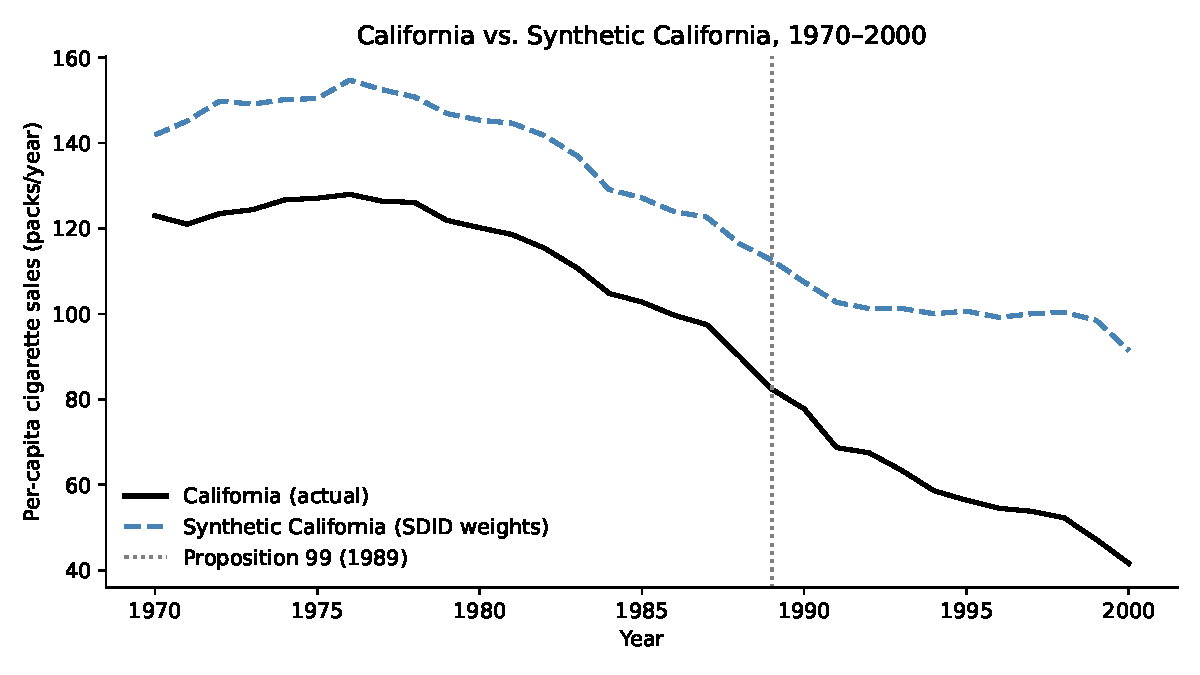
\includegraphics[width=0.85\textwidth]{../output/figures/sdid_trends.pdf}
    \caption{Actual vs.\ synthetic California per-capita cigarette sales, 1970--2000.
    The synthetic California is the SDID-weighted average of 38 donor states.
    The vertical dotted line marks Proposition 99 (1989).}
    \label{fig:trends}
\end{figure}

SDID, SC, DID, and DIFP estimates all match the paper closely.
The DIFP estimate is consistent with the paper's $-11.1$: using uniform time weights
combined with demeaned SC unit weights produces a smaller (in absolute value)
estimate than plain SC because the pre-treatment trend is subtracted out.
The MC estimate is not replicated; see Section~\ref{sec:challenges}.

California's Proposition 99 reduced annual per-capita cigarette consumption by
approximately $15.6$ packs per person per year over 1989--2000 under the most
credible estimator (SDID).
The wide range across methods illustrates how sensitive causal estimates are to the
choice of estimator, and motivates the paper's theoretical and empirical case for SDID.

\section{Challenges in Replication}
\label{sec:challenges}

\paragraph{No official Python package; limited replication support.}
The original authors released only an R package
(\texttt{synth-inference/synthdid} on GitHub) and provide no official Python
implementation, no installation instructions for Python users, and no guidance on
which regularization formula to use when implementing from scratch.
Two third-party Python ports exist --- \texttt{pysynthdid} (by Masa Asami)
and a PyPI package called \texttt{synthdid} --- but neither is affiliated
with the original authors.
The PyPI package failed to install entirely due to a dependency on numpy~1.23.5,
which is incompatible with Python~3.13.
The \texttt{pysynthdid} package installed successfully but illustrates a subtler
problem: it selects the regularization parameter $\zeta_\omega$ via
\emph{Bayesian optimization} rather than the analytical formula
$\zeta_\omega = (N_{\text{tr}} T_{\text{post}})^{1/4} \hat{\sigma}$
specified in the paper.
This methodological difference means that even a working Python port does not
reproduce the paper's point estimates without careful inspection of source code;
\texttt{pysynthdid} returns an SDID estimate of approximately $-19.8$
(compared to the paper's $-15.6$), a gap driven entirely by the different
regularization approach.
A researcher wishing to replicate this paper in Python must therefore read the
authors' R source code line-by-line and re-implement the algorithm from scratch,
or accept results that silently differ from those in the paper.
This replication implements the Frank-Wolfe algorithm directly from
\texttt{R/solver.R} and \texttt{R/synthdid.R}.

\paragraph{MC estimator requires a separate R package.}
The paper's MC estimate uses \texttt{mcnnm\_cv} from the \texttt{MCPanel} R package,
which performs cross-validated nuclear norm minimization with unit and time fixed effects.
No equivalent Python package exists, and porting the algorithm fully would require
implementing cross-validated proximal gradient descent with two-way fixed effects.
MC is therefore not replicated.

\paragraph{Non-standard data delimiter.}
The CSV file (\texttt{input/california\_prop99.csv}) uses a semicolon separator
rather than a comma, which causes a silent parsing failure with default settings.

\paragraph{Computationally intensive standard errors.}
The placebo SE re-runs full Frank-Wolfe optimization for each replication.
200 replications per estimator required approximately 45 seconds per run.

One important lesson from the replication process is that \textbf{when a paper
depends on multiple packages across different languages, full replication
requires either porting each dependency or accepting partial discrepancies ---
making transparent documentation of those discrepancies a necessary part
of any honest replication exercise}.

\section{What I Learned}

The easiest part of this replication was the mathematical translation: the
Frank-Wolfe weight estimation procedure is described precisely in the paper and
maps cleanly to NumPy operations once the collapsed-form matrix construction
and exact line search are understood.
DID and DIFP required only understanding the weight structures, not
any new optimization.

The hardest part was discovering that \emph{no working Python implementation
exists that faithfully reproduces the paper's results}.
The R-only official package, the broken PyPI port, and the methodological
divergence in \texttt{pysynthdid} all had to be diagnosed before any
replication could begin.
This surface is invisible from reading the paper itself, which presents the
estimator mathematically and points to an R package --- a reader using Python
would not know until they attempt installation that both available ports are
either broken or divergent.

This experience revealed a structural gap in how the paper supports replication:
the code deposit at OpenICPSR contains only R scripts, and the paper provides no
cross-language guidance.
A simple note in the replication materials identifying which regularization
formula \texttt{pysynthdid} uses --- and why it differs from the paper's ---
would have saved several hours of debugging and would have made the Python
replication path accessible without reading the R source.
More broadly, as empirical economics increasingly spans Python and R user bases,
releasing replication packages in only one language creates a reproducibility
barrier that is invisible to authors but significant for readers.

\bibliographystyle{apalike}
\bibliography{references}

\end{document}
